\chapter{Cài đặt và quản lý module trong NodeJS}
\section{Cài đặt NodeJS}
	\subsection{Cài đặt NodeJS}
   Để cài đặt NodeJS bạn có thể truy cập và trang \url{http://nodejs.org/download/} để tải phiên bản phù hợp với hệ điều hành của bạn xuống.
      \textbf{Với Windows:} \\
		Bạn chỉ cần chạy file \textit{node-v0.8.18-x84.msi} hoặc \textit{node-v0.8.18-x64.msi} tùy theo hệ điều hành đang sử dụng và tiến hành cài đặt bình thường.

	\begin{figure}[-h]
		\centering
		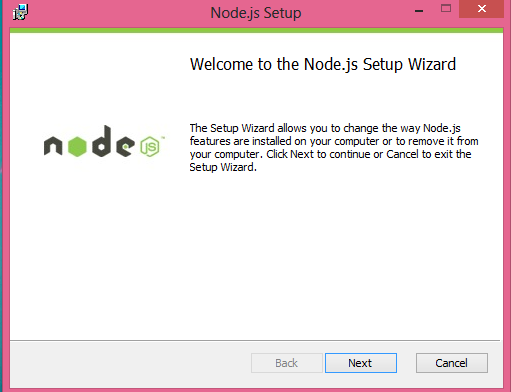
\includegraphics[scale=0.7]{2_1}
	\end{figure}
	
	\begin{figure}[-h]
		\centering
		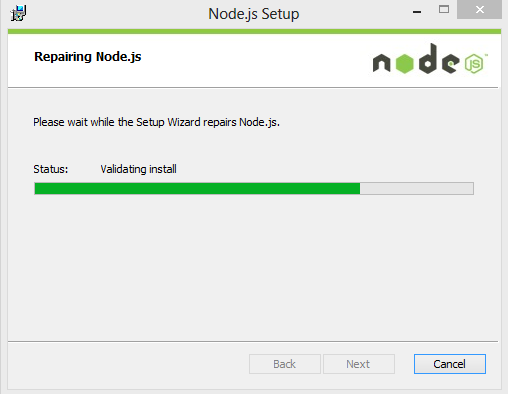
\includegraphics[scale=0.7]{2_2}
	\end{figure}

	\textbf{Với Linux:}\\
		 Sau khi tải về gói package của NodeJs ta tiến hành thực hiện các bước sau:\\
			\begin{enumerate}
				\item \$ \texttt{xzf node-v0.8.18.tar.gz}
				\item \$ \texttt{cd node -v0.8.18}
				\item \$ \texttt{./configure}
				\item \$ \texttt{make}
				\item \$ \texttt{sudo make install}
			\end{enumerate}
		 Ngoài ra một số bản phân phối linux cho phép bản tải NodeJS thông qua package. Để thực hiện điều đó, bạn chỉ cần vào terminal và gõ lệnh:\\
						\fbox{\texttt{\$ apt-get install nodejs}}		

	Để kiểm tra máy đã cài nodeJS chưa ta thực hiện lệnh:\\
					\fbox{\texttt{\$ node -v}}

	\subsection{Sử dụng NodeJs}
Sau khi tiến hành cài đặt xong NodeJs chúng ta bắt đầu sử dụng Node. Để khởi động giao diện dòng lệnh của Node ta sử dụng câu lệnh: \\
	\texttt{\$ node}

Tiến hành kiểm tra việc cài đặt và quan sát Node đang làm gì, ta sử dụng: \\
	\texttt{> console.log('Hello World!')}\\
	\texttt{Hello World!} \\
	\texttt{> undefined} \\

Cũng có thể chạy một JavaScript từ một file. Nếu tạo chúng ta tạo một file \texttt{hello\_world.js} với nội dung.\\
	\texttt{console.log('Hello World!')}\\

Tiến hành file trên với câu lệnh:\\
	\texttt{\$ node hello\_world.js} \\
	\texttt{Hello World}
\section{Quản lý module trong NodeJS}
	\subsection{Quản lý module trong NodejS}
		Với NodeJs ta có thể mở rộng các chức năng hông qua các module. Để quản lý chúng, ta sử dụng một phần mềm của bên thứ 3 là \textit{npm} (Node Package control management). Thông tin về \textit{npm} có thể tìm thấy ở trang chủ :  \url{http://npmjs.org}.
	 Npm được cài sẵn khi cài Nodejs.
	\begin{enumerate}
		
			\item Để liệt kê các gói ta sử dụng lệnh \\
					\fbox{\texttt{\$ node ls [filter]}}
				\begin{itemize}
					\item Liệt kê tất cả các gói \\
						\texttt{\$ node ls}
					\item Liệt kê tất cả các gói được cài đặt \\
						\texttt{\$ node ls installed}					
					\item Liệt kê tất cả các gói đang ở trạng thái ổn định(stable)\\
						\texttt{\$ node ls stable}						
					\item Liệt kê tất cả các gói theo tên \\
						\texttt{\$ node ls "tên hoặc pattern"}
				\end{itemize}
			
			\item Để cài đặt gói ta sử dụng lệnh:\\
					\fbox{\texttt{\$ npm install package[@filters]}}
				\begin{itemize}
					\item Cài gói express \\
						\texttt{\$ npm install express}
					\item Cài gói express phiên bản 2.0.0beta \\
						\texttt{\$ npm install  express@2.0.0beta}						
					\item Cài gói phiên bản lớn hơn 0.1.0 \\
						\texttt{\$ npm install express@">=0.1.0}
				\end{itemize}
			\item Để gỡ một gói , ta dùng lệnh \\
				\fbox{\texttt{\$	npm rm [-g] <package name>[@version]}}
			\item Để xem thông tin về module nào đó ta sử dụng lệnh. \\
				\fbox{\texttt{\$ npm view [@] [[.]...]}}
			\item Để update các module bằng việc sử dụng câu lệnh:\\
	\fbox{\texttt{\$ npm update [-g] <package name>}}
		\end{enumerate}
	\section{Xây dựng và sử dụng các module}
	Trong phần này, ta sẽ tìm hiểu cách xây dựng và sử dụng một module cho nodeJS.

			\begin{minted}[linenos=true, tabsize=4]{javascript}
var module = require(path_to_module| module_name);
			\end{minted}
			
	Tham số truyền vào là tên module nếu đó là một core module được quản lý qua npm. Trong trường hợp module đó là một module custom của người dùng, ta chỉ cần chi ra đường dẫn đến file đó. 

	Ngoài ra ta cũng có thể load các module trong một thư mục. Đầu tiên Nodejs sẽ kiểm tra xem đó có phải là một packge hay không thông qua kiểm tra một file package.json. Cấu trúc file json sẽ chứa thông tin về file chính của package. Ví dụ:
			
			\begin{minted}[linenos=true, tabsize=4]{javascript}
{
	"name": "myModule",
	"main": "./lib/myModule.js"	
}			
			\end{minted}
	
	Khi đó, Node sẽ thử load file path\_to\_module/lib/myModule.js
	
	Một điểm quan trọng cần lưu tâm là khi thực hiện thao tác này, ta đã cache module đó. Do vậy khi viết nhiều lần nạp module, thực chất chỉ có một hàm đã được thực hiện.
	Để truy cập vào các thành phần của module, module cần phải xuất thông tin đó ra thông qua lệnh module.exports.\\
		Ví dụ: 	
		
		\begin{minted}[linenos=true, tabsize=4]{javascript}
//test.js
var level = 0;

function loadGame(){
         //code in here
}

function playGame(){
        //code in here
}

module.exports.loadGame = loadGame;
module.exports.playGame = payGame;
module.exports.level = level;

//app.js
var test = require('./test.js');
test.loadGame();
test.playGame();
console.log(test.level);
		\end{minted}
		
		Trong ví dụ này, trong module test, ta đã xuất ra thông tin gồm 2 hàm và một biến. Chính vì vậy khi load module này vào file app.js, ta có thể sử dụng chúng.
